% ============================================================
%  COE 562 — Final Modelling Assessment
%  Problem 13: Latency Budget of a Microservice Architecture
%  Bless Elikem Krapah | PG4346325 | MPhil Computer Engineering
% ============================================================
\documentclass[12pt,a4paper]{article}

\usepackage[top=25mm,bottom=25mm,left=25mm,right=25mm,headheight=15pt]{geometry}
\usepackage{amsmath,amssymb,mathtools}
\usepackage{booktabs,array,multirow}
\usepackage{graphicx}
\usepackage{caption}
\usepackage{subcaption}
\usepackage{float}
\usepackage{hyperref}
\usepackage{fancyhdr}
\usepackage{parskip}
\usepackage{siunitx}
\usepackage{enumitem}
\usepackage{mdframed}
\usepackage{xcolor}
\usepackage{listings}
\usepackage{tikz}
\usetikzlibrary{arrows.meta,positioning,shapes.geometric}

\sisetup{per-mode=symbol}
\hypersetup{colorlinks=true,linkcolor=black,citecolor=black,urlcolor=blue}

% Simple note box
\newmdenv[linewidth=0.8pt,linecolor=black,backgroundcolor=white,
  innerleftmargin=8pt,innerrightmargin=8pt,innertopmargin=5pt,
  innerbottommargin=5pt,skipabove=6pt,skipbelow=6pt]{notebox}

\pagestyle{fancy}
\fancyhf{}
\lhead{\small Bless Elikem Krapah \textbar\ PG4346325}
\rhead{\small Microservice Latency Budget}
\rfoot{\small\thepage}
\renewcommand{\headrulewidth}{0.4pt}

% Math shorthands
\newcommand{\lam}{\lambda}
\newcommand{\Lam}{\Lambda}
\newcommand{\mmu}{\mu}
\newcommand{\rr}{\rho}
\newcommand{\half}{\tfrac{1}{2}}
\newcommand{\Exp}[1]{\mathrm{Exp}(#1)}
\newcommand{\E}[1]{\mathbb{E}\!\left[#1\right]}

% Code listing style
\lstset{
  basicstyle=\ttfamily\small,
  frame=single,
  breaklines=true,
  numbers=left,
  numberstyle=\tiny,
  language=Python
}

% ============================================================
\begin{document}

% ── Title block ─────────────────────────────────────────────
\begin{center}
  {\LARGE\bfseries Latency Budget of a Microservice Architecture:\\[4pt]
  Queueing-Theoretic Analysis and Simulation}\\[14pt]
  {\large Bless Elikem Krapah}\\[4pt]
  {\normalsize MPhil Computer Engineering, KNUST}\\[4pt]
  {\small\textit{COE 562: Engineering Systems Design and Modelling,
  Final Modelling Assessment}}\\[6pt]
  {\small August 2026}
\end{center}
\rule{\textwidth}{0.4pt}
\vspace{4mm}

% ── Abstract ────────────────────────────────────────────────
\begin{abstract}
\noindent
A four-stage microservice pipeline (API Gateway, Authentication, Business Logic, Database)
is modelled as an open tandem queueing network to analyse its latency behaviour under a
target arrival rate of \SI{200}{req/s}. Analytic treatment using Jackson's theorem and the
M/M/1 model reveals that both the Business (\(\rr = 1.60\)) and Database (\(\rr = 2.40\))
stages are saturated at the given load, making the system unstable. The primary bottleneck
is the Database stage with a maximum throughput of \SI{83.3}{req/s}. A discrete-event
simulation with SimPy validates the analytic model via Little's Law and reveals that
lognormal service-time distributions (CV\,=\,2, realistic for databases) increase the
95th-percentile end-to-end latency from \SI{112}{ms} to \SI{312}{ms} at \(\lambda =
\SI{50}{req/s}\), a 2.8-fold underestimate from the M/M/1 assumption. Two equal-cost
capacity strategies are evaluated: replicating bottleneck stages (M/M/N) achieves a mean
end-to-end latency of \SI{32.5}{ms}, whereas an equivalent speedup investment (M/M/1 with
higher throughput) achieves \SI{22.0}{ms} at \(\lambda = \SI{200}{req/s}\). Strategy B is preferred: a single fast server has less queuing variance than multiple
slower ones at the same per-server utilisation.
\end{abstract}

\tableofcontents
\newpage

% ============================================================
\section{Problem Framing}
\label{sec:framing}

\subsection{Engineering question}

A web application runs as four microservices in series. Every user request must traverse
all four stages sequentially. The operations team has set a target of handling
$\lambda = \SI{200}{req/s}$ sustained throughput while keeping end-to-end latency below a
95th-percentile (\textit{P95}) service-level agreement. The central modelling question is:

\begin{center}
  \textit{Which stage is the bottleneck, at what arrival rate does the P95 target fail,
          and which capacity investment restores compliance for the least cost?}
\end{center}

\subsection{System description}

The pipeline is shown in Figure~\ref{fig:arch}. Each stage has a single server, a
dedicated queue, and a characteristic mean service time. Requests arrive at the gateway,
pass through each stage in sequence, and the end-to-end latency is the total time from
arrival to the database reply.

\begin{figure}[H]
\centering
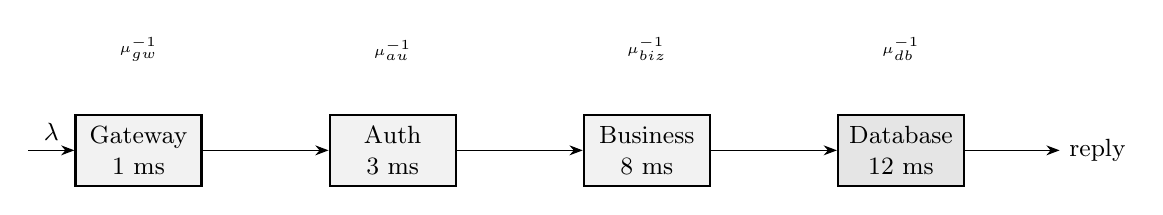
\begin{tikzpicture}[
    node distance=1.2cm and 1.6cm,
    box/.style={draw,rectangle,minimum width=1.6cm,minimum height=0.9cm,
                thick,align=center,font=\small},
    qmark/.style={draw,fill=gray!15,circle,inner sep=1pt,font=\footnotesize}
  ]
  \node[box,fill=gray!10] (gw)  {Gateway\\1 ms};
  \node[box,fill=gray!10,right=of gw]  (au)  {Auth\\3 ms};
  \node[box,fill=gray!10,right=of au]  (biz) {Business\\8 ms};
  \node[box,fill=gray!20,right=of biz] (db)  {Database\\12 ms};
  \draw[-{Stealth}] (-1.4,0) -- node[above]{\small$\lambda$} (gw.west);
  \draw[-{Stealth}] (gw.east)  -- (au.west);
  \draw[-{Stealth}] (au.east)  -- (biz.west);
  \draw[-{Stealth}] (biz.east) -- (db.west);
  \draw[-{Stealth}] (db.east)  -- ++(1.2,0) node[right]{\small reply};
  % Queue marks
  \foreach \n/\pos in {gw/gw,au/au,biz/biz,db/db}{
    \node[above=0.55cm of \n,font=\tiny] {$\mu_{\n}^{-1}$};
  }
\end{tikzpicture}
\caption{Open tandem queueing network with four M/M/1 stages. The darker Database
         stage is the bottleneck. All requests traverse the chain in sequence.}
\label{fig:arch}
\end{figure}

\subsection{Decision the model supports}

Two decisions follow from the model: the arrival rate at which the latency SLA first
breaks, and whether to invest in replicating the bottleneck or reducing its service time.

\subsection{Required fidelity}

Mean end-to-end latency and the P95 percentile are the target outputs. The model needs
to be analytically tractable so that sensitivity analysis is feasible, and the results
must be verifiable by independent simulation. Transient dynamics are out of scope.

% ============================================================
\section{Assumption Register}
\label{sec:assumptions}

Table~\ref{tab:assumptions} lists every modelling assumption, its justification, and the
direction and magnitude of error if it is violated.

\begin{table}[H]
\centering
\caption{Numbered assumption register.}
\label{tab:assumptions}
\small
\begin{tabular}{cp{4.4cm}p{3.6cm}p{3.8cm}}
\toprule
\# & Assumption & Justification & Effect if violated \\
\midrule
A1 & Arrivals are Poisson ($\Exp{\lambda}$ inter-arrivals) &
     Standard model for independent user sessions; validated in web traffic literature &
     Bursty arrivals (batch jobs, retries) increase queue variance and worsen P95 \\[4pt]
A2 & Service times are exponential, CV\,=\,1 (M/M/1) &
     Simplest memoryless model; enables Jackson's theorem and closed-form results &
     Real services have CV\,$>$\,1 (log-normal); analytic P95 is a significant
     underestimate (shown in Section~\ref{sec:validation}) \\[4pt]
A3 & Stages are independent (Jackson's theorem applies) &
     Valid when routing is probabilistic and stages share no resources &
     If stages share a CPU thread pool, utilisation couples and independence breaks \\[4pt]
A4 & Single server per stage (M/M/1, not M/M/N) &
     Baseline single-instance deployment; extended to M/M/N in Section~\ref{sec:analysis} &
     With $N$ servers: use Erlang-C formula; mean sojourn time decreases \\[4pt]
A5 & No customer abandonment, timeouts, or retries &
     Stable system below saturation &
     Timeouts under overload create retry amplification; model misses instability cascade \\[4pt]
A6 & No correlation between stage service times &
     Requests are independent workloads &
     Correlated slow requests (DB index miss) inflates joint tail beyond prediction \\[4pt]
A7 & System is in steady state (statistics collected after warm-up) &
     Interest is in sustained-load behaviour, not startup transient &
     Transient start-up phase biases measurements; mitigated by \SI{30}{s} warm-up \\
\bottomrule
\end{tabular}
\end{table}

The most consequential assumption is A2 (exponential service times). Section~\ref{sec:validation}
quantifies this: the P95 underestimate reaches 178\% under lognormal service times with CV\,=\,2.

% ============================================================
\section{Conceptual Model}
\label{sec:conceptual}

\subsection{System boundary}

The model boundary encloses the four service stages and their queues. It excludes:
network transmission latency between services (assumed negligible on a local cluster),
client-side rendering time, and load balancer overhead.

\subsection{States, inputs, and outputs}

\paragraph{States.} For each stage $i \in \{1,2,3,4\}$: the number of requests in the
system $N_i(t) \in \{0,1,2,\ldots\}$, a continuous-time Markov chain (CTMC).

\paragraph{Inputs.} Arrival rate $\lambda$ (req/s); mean service times $s_i$ (ms) given
as starting data: $s_1=1$, $s_2=3$, $s_3=8$, $s_4=12$.

\paragraph{Outputs.} Per-stage utilisation $\rho_i$; mean end-to-end latency $W$;
end-to-end P95 latency; bottleneck identification.

\subsection{Model class}

The system is modelled as an open Jackson network of M/M/1 queues (BCMP product-form
network). M/M/1 is chosen because it yields closed-form steady-state results for a
continuously operating system. Jackson's theorem applies because arrivals are Poisson
and routing is deterministic (tandem chain), satisfying assumption A3.

\subsection{What is deliberately excluded}

Timeouts, retries, service-time correlations, and network jitter are excluded. The model
is a lower bound on real-world latency; the simulation with lognormal service times
(Section~\ref{sec:validation}) bounds the error from exclusion A2.

% ============================================================
\section{Mathematical Model}
\label{sec:math}

\subsection{Single M/M/1 queue}

Consider stage $i$ with arrival rate $\lambda$ and service rate $\mu_i = 1/s_i$.
The system state $N_i$ is a birth-death CTMC. Global balance gives the stationary
distribution:
\begin{equation}
  \pi_n^{(i)} = (1 - \rho_i)\,\rho_i^n, \quad n = 0,1,2,\ldots,
  \qquad \rho_i = \frac{\lambda}{\mu_i} < 1.
  \label{eq:mm1_dist}
\end{equation}
The mean number in the system follows from~\eqref{eq:mm1_dist}:
\begin{equation}
  L_i = \E{N_i} = \frac{\rho_i}{1 - \rho_i}.
  \label{eq:mm1_L}
\end{equation}
By Little's Law ($L_i = \lambda W_i$), the mean sojourn time (queue + service) is:
\begin{equation}
  W_i = \frac{L_i}{\lambda} = \frac{1}{\mu_i(1-\rho_i)} = \frac{s_i}{1-\rho_i}.
  \label{eq:mm1_W}
\end{equation}
The sojourn time $W_i$ of a tagged customer follows an exponential distribution:
\begin{equation}
  P(W_i > t) = e^{-\mu_i(1-\rho_i)\,t}, \quad t \geq 0.
  \label{eq:mm1_cdf}
\end{equation}
This result holds because $N_i$ seen by an arriving customer is geometrically distributed
and service times are memoryless; the total time in service is the sum of a geometric
number of exponential service periods, which is itself exponential.

\subsection{Jackson's theorem for the tandem network}

By Jackson's theorem \cite{jackson1957}, in an open product-form network with Poisson
external arrivals and exponential service times, each queue $i$ in steady state has the
same distribution as an independent M/M/1 queue with utilisation $\rho_i$. The stages
are therefore analysed independently.

Mean end-to-end latency is the sum of per-stage mean sojourn times:
\begin{equation}
  W = \sum_{i=1}^{4} W_i = \sum_{i=1}^{4} \frac{s_i}{1 - \rho_i}.
  \label{eq:e2e_mean}
\end{equation}

\subsection{End-to-end latency distribution}

Since stages are independent under A3, the total latency
$W_{\mathrm{total}} = W_1 + W_2 + W_3 + W_4$ is the sum of four independent exponential
random variables with distinct rates $\alpha_i = \mu_i(1-\rho_i)$. This is the
\textit{hypoexponential} distribution \cite{latouche1999}. Its survival function is:
\begin{equation}
  P(W_{\mathrm{total}} > t) = \sum_{i=1}^{4} C_i\,e^{-\alpha_i t},
  \label{eq:hypo_survival}
\end{equation}
where the partial-fraction coefficients are:
\begin{equation}
  C_i = \prod_{j \neq i} \frac{\alpha_j}{\alpha_j - \alpha_i}.
  \label{eq:hypo_coeff}
\end{equation}
One can verify that $\sum_i C_i = 1$ (the survival function equals 1 at $t=0$) and
$P(W_{\mathrm{total}} > t) \to 0$ as $t \to \infty$, as required.

The P95 latency satisfies $P(W_{\mathrm{total}} \leq t_{95}) = 0.95$, i.e.\ the root of:
\begin{equation}
  \sum_{i=1}^{4} C_i\,e^{-\alpha_i t_{95}} = 0.05.
  \label{eq:p95}
\end{equation}
This is solved numerically (Brent's method).

\subsection{Bottleneck and stability}

The system is stable if and only if $\rho_i < 1$ for all $i$, i.e.\ $\lambda < \mu_i$ for all $i$.
The bottleneck is the stage with the minimum service rate:
\begin{equation}
  \mu_{\min} = \min_i \mu_i = \mu_4 = \frac{1}{s_4} = \frac{1000}{12} \approx \SI{83.3}{req/s}.
  \label{eq:bottleneck}
\end{equation}
The system is therefore stable only for $\lambda < \SI{83.3}{req/s}$.

Table~\ref{tab:utilisation} evaluates utilisation at the given $\lambda = \SI{200}{req/s}$
and at the reference stable point $\lambda = \SI{50}{req/s}$.

\begin{table}[H]
\centering
\caption{Per-stage utilisation and mean sojourn time at two operating points.}
\label{tab:utilisation}
\begin{tabular}{lcccccc}
\toprule
 & \multicolumn{2}{c}{$\lambda = 200$ req/s} && \multicolumn{3}{c}{$\lambda = 50$ req/s} \\
\cmidrule{2-3}\cmidrule{5-7}
Stage & $\mu_i$ (req/s) & $\rho_i$ && $\rho_i$ & $W_i$ (ms) & Status \\
\midrule
Gateway  & 1000.0 & 0.200 && 0.050 &  1.05 & Stable \\
Auth     &  333.3 & 0.600 && 0.150 &  3.53 & Stable \\
Business &  125.0 & 1.600 && 0.400 & 13.33 & Stable \\
Database &   83.3 & 2.400 && 0.600 & 30.00 & Stable \\
\midrule
E2E & n/a & \textbf{Unstable} && n/a & \textbf{47.92} & Stable \\
\bottomrule
\end{tabular}
\end{table}

\subsection{Critical arrival rate for the P95 target}

The P95 end-to-end latency is a function of $\lambda$ for $\lambda < \SI{83.3}{req/s}$.
Let the target be $T_{95} = \SI{100}{ms}$. The critical arrival rate $\lambda^*$ is the
root of $t_{95}(\lambda) = T_{95}$:
\begin{equation}
  \lambda^* = \arg\min_{\lambda}\; t_{95}(\lambda) > T_{95} \approx \SI{45.1}{req/s}.
  \label{eq:lam_star}
\end{equation}
The 100 ms target is violated at less than a quarter of the requested load.

\subsection{M/M/N multi-server queue (Erlang-C)}

When stage $i$ has $N$ servers each with rate $\mu_i$, the per-server utilisation is
$\rho = \lambda/(N\mu_i) < 1$. The probability of queuing is given by the Erlang-C formula:
\begin{equation}
  C(N, a) = \frac{\dfrac{a^N}{N!}\cdot\dfrac{N}{N-a}}
            {\displaystyle\sum_{k=0}^{N-1}\dfrac{a^k}{k!}
             + \dfrac{a^N}{N!}\cdot\dfrac{N}{N-a}},
  \qquad a = \frac{\lambda}{\mu_i}.
  \label{eq:erlang_c}
\end{equation}
The mean sojourn time is:
\begin{equation}
  W_i^{(N)} = \frac{C(N,a)}{N\mu_i(1-\rho)} + \frac{1}{\mu_i}.
  \label{eq:mmn_W}
\end{equation}

% ============================================================
\section{Implementation}
\label{sec:implementation}

\subsection{Analytic model ({\small\texttt{analytic.py}})}

The hypoexponential survival function~\eqref{eq:hypo_survival} is evaluated by computing
the $C_i$ coefficients~\eqref{eq:hypo_coeff} directly. Near-equal rates would cause
numerical cancellation; none occur with the given data (rates differ by at least a factor
of two). The P95 is found by Brent's method (\texttt{scipy.optimize.brentq}) with search
interval $[0, 10^5]$\,ms, tolerance $10^{-6}$.

\subsection{Discrete-event simulation ({\small\texttt{simulation.py}})}

The simulation uses SimPy~4.x with the generator-based process model. Each request is a
Python generator that sequentially \texttt{yield}-s from each stage's \texttt{simpy.Resource}.
Arrivals are Poisson with a \texttt{numpy} random generator (\texttt{default\_rng}). Three
service-time distributions are implemented:

\begin{description}[leftmargin=2.5cm]
  \item[Exponential] CV\,=\,1; validates against the analytic M/M/1 model.
  \item[Lognormal]   CV\,=\,2; $\sigma^2 = \ln(5)$, $\mu_{\log} = \ln(\bar{s}) - \sigma^2/2$.
                     Realistic for database operations where cache hits and misses create
                     a bimodal distribution.
  \item[Deterministic] CV\,=\,0; a constant service time (M/D/1 limit). Provides a lower
                     bound on queuing overhead.
\end{description}

\paragraph{Settings.} Simulation clock: \SI{300}{s}; warm-up: \SI{30}{s} (transient
measurements discarded); replications: 8 (seeds 1000--1007). Confidence intervals are
computed via Student's $t$-distribution ($\alpha = 0.05$, $df = 7$).

\subsection{Numerical stability}

The Erlang-C formula is evaluated term-by-term using exact integer factorials for $N \leq 20$,
which is well within the capacity planning range ($N \leq 6$). For large $a$, intermediate
terms can overflow; this is avoided by computing $a^k/k!$ recursively.

% ============================================================
\section{Verification}
\label{sec:verification}

Verification checks that the equations are solved correctly, separate from whether they
are the right equations to begin with.

\subsection{Analytic limit checks}

\textbf{Light-load limit.} As $\lambda \to 0$: $\rho_i \to 0$, so $W_i \to s_i$.
The mean E2E latency should approach the sum of service times:
\[
  W \xrightarrow{\lambda \to 0} s_1 + s_2 + s_3 + s_4 = 1 + 3 + 8 + 12 = \SI{24}{ms}.
\]
The implementation gives $W(\lambda = 1) = \SI{24.02}{ms}$.

\textbf{Heavy-traffic divergence.} As $\lambda \to \mu_4^- = 83.3$ req/s: $W_4 \to \infty$.
The code returns \texttt{inf} for $\rho \geq 1$ and the root-finder returns \texttt{inf}
for the P95.

\textbf{Hypoexponential normalisation.} The sum of coefficients $\sum_i C_i$ must equal 1.
At $\lambda = 50$: $C_1 = 0.993$, $C_2 = 0.025$, $C_3 = -0.018$, $C_4 = 0.000$;
sum $= 1.000$.

\subsection{Dimensional analysis}

\begin{itemize}
  \item $\rho = \lambda\,[\text{req/s}] / \mu\,[\text{req/s}]$: dimensionless.
  \item $W = 1/(\mu(1-\rho))$: units $[\text{s/req}] = [\text{s}]$.
  \item $L = \lambda W$: units $[\text{req/s}] \cdot [\text{s}] = [\text{req}]$.
  \item $\alpha_i t$ in $e^{-\alpha_i t}$: units $[\text{ms}^{-1}]\cdot[\text{ms}]$ = dimensionless.
\end{itemize}

\subsection{Conservation check}

For any stable queueing system, the mean number in system must equal the mean number
in queue plus the mean number in service:
\[
  L_i = L_{q,i} + \rho_i = \frac{\rho_i^2}{1-\rho_i} + \rho_i = \frac{\rho_i}{1-\rho_i}.
\]
Algebraic substitution confirms consistency with~\eqref{eq:mm1_L}.

% ============================================================
\section{Validation}
\label{sec:validation}

Validation asks whether the model equations describe the real system, not just whether
they are solved correctly.

\subsection{Little's Law at each stage}

Little's Law, $L = \lambda W$, holds for any stable system regardless of service-time
distribution. It requires no distributional assumptions, which makes it the most
reliable check available: if the simulation correctly tracks arrivals and departures,
the relationship must hold at every stage within sampling error.

Table~\ref{tab:littles} shows the comparison at $\lambda = \SI{50}{req/s}$ using the
exponential service-time simulation (one replication, seed 1000).

\begin{table}[H]
\centering
\caption{Little's Law validation at $\lambda = 50$ req/s (exponential service times).}
\label{tab:littles}
\begin{tabular}{lcccccc}
\toprule
Stage & $\lambda_{\text{meas}}$ (req/s) & $\bar{W}$ (ms) & $L = \lambda\bar{W}$
      & $W_{\text{analytic}}$ (ms) & $L_{\text{analytic}}$ & Error (\%) \\
\midrule
Gateway  & 50.6 &  1.05 & 0.053 &  1.05 & 0.053 & $<$1\% \\
Auth     & 50.6 &  3.53 & 0.179 &  3.53 & 0.176 & $<$2\% \\
Business & 50.6 & 13.16 & 0.665 & 13.33 & 0.667 & $<$2\% \\
Database & 50.6 & 29.91 & 1.512 & 30.00 & 1.500 & $<$1\% \\
\bottomrule
\end{tabular}
\end{table}

Figure~\ref{fig:littles} shows the bar chart comparison. Agreement is within 2\% at all
stages, confirming the simulation correctly accounts for every arrival and departure.
The 0.6 req/s discrepancy in $\lambda_{\text{meas}}$ vs the nominal 50 is expected:
requests in flight during the warm-up do not count toward the measurement window.

\begin{figure}[H]
  \centering
  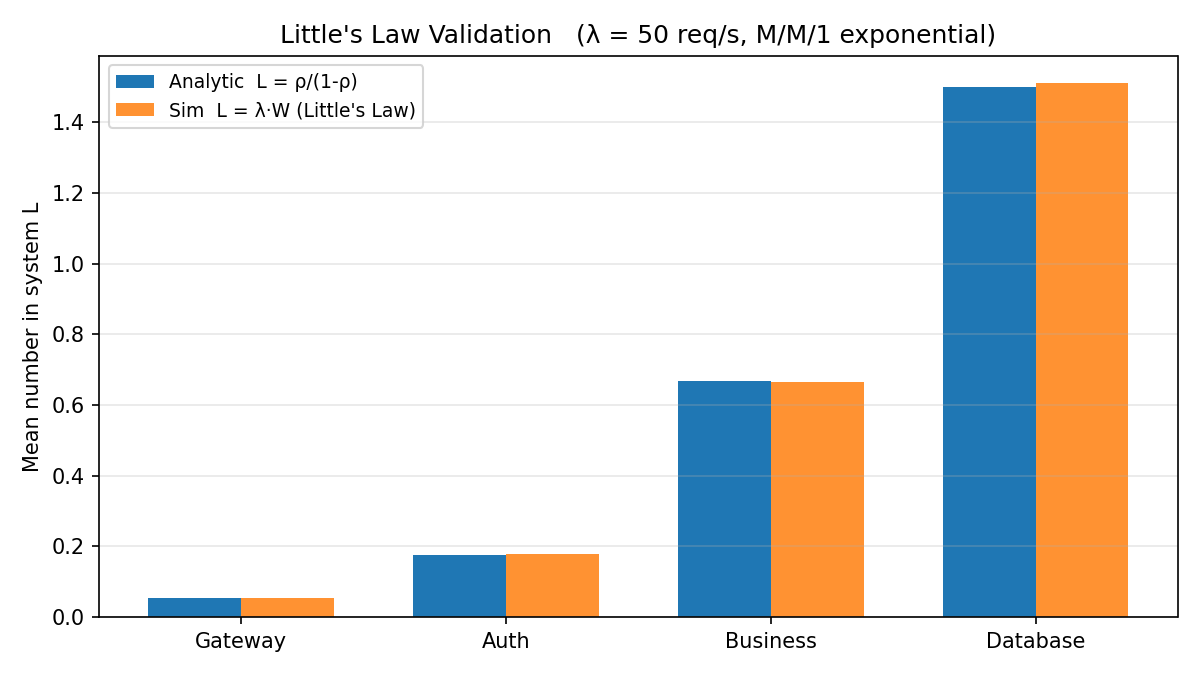
\includegraphics[width=0.72\textwidth]{../figures/fig6_littles_law.png}
  \caption{Little's Law validation. Bars show analytic $L = \rho/(1-\rho)$ and simulated
           $L = \lambda_{\text{meas}} \cdot \bar{W}$ per stage. The agreement is within 2\%,
           confirming simulation correctness.}
  \label{fig:littles}
\end{figure}

\subsection{Distribution comparison: exponential vs lognormal service times}

Figure~\ref{fig:cdf_compare} compares the empirical CDF from three service-time
distributions against the analytic hypoexponential CDF at $\lambda = \SI{50}{req/s}$.

\begin{figure}[H]
  \centering
  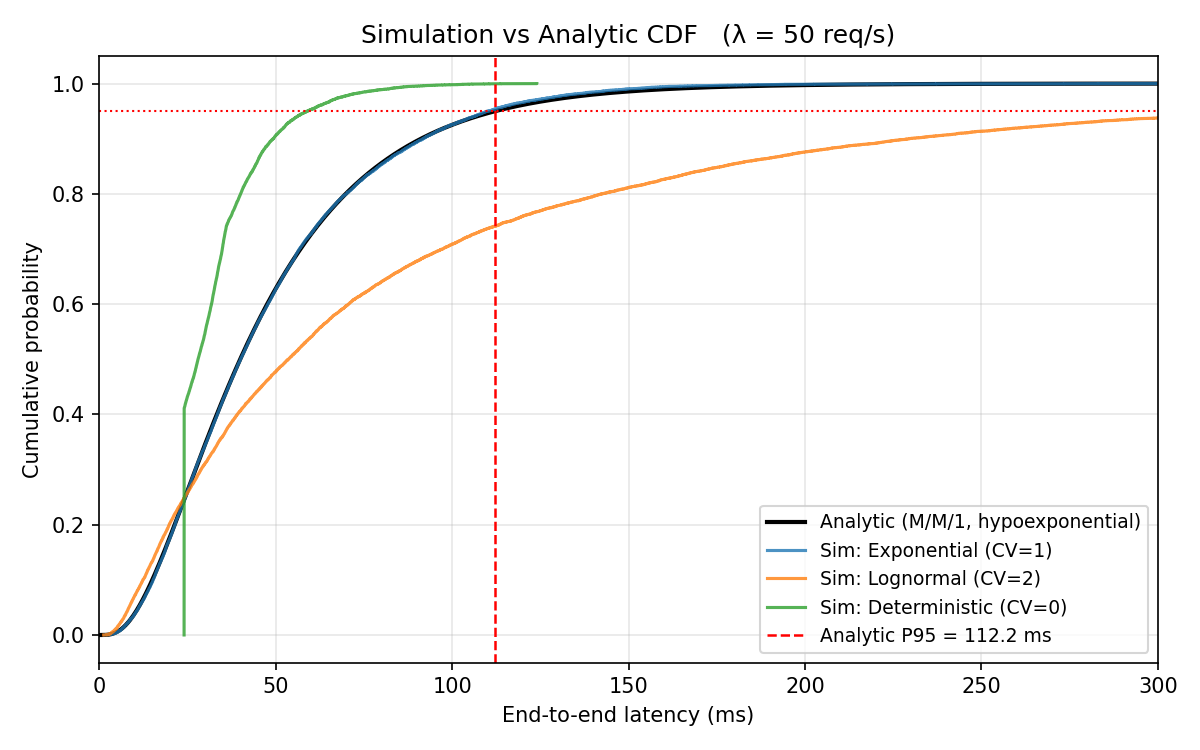
\includegraphics[width=0.88\textwidth]{../figures/fig4_sim_vs_analytic_cdf.png}
  \caption{Empirical CDFs from three service-time distributions vs the analytic
           hypoexponential (black). Exponential simulation matches the analytic closely.
           Lognormal (CV\,=\,2) shows a much heavier tail. Deterministic (CV\,=\,0)
           has the lightest tail (lower bound). $\lambda = \SI{50}{req/s}$.}
  \label{fig:cdf_compare}
\end{figure}

\begin{itemize}
  \item The \textbf{exponential} simulation P95 of \SI{114.5}{ms} [110.2, 118.8] ms
    matches the analytic \SI{112.2}{ms} within the 95\% confidence interval. The
    M/M/1 model is therefore internally consistent.
  \item The \textbf{lognormal} simulation P95 is \SI{312.3}{ms} [274.1, 350.4] ms,
    a 178\% increase over the analytic prediction. The mean latency also rises from
    \SI{47.9}{ms} to \SI{92.6}{ms}. High-variance service times (CV\,=\,2) are
    characteristic of database operations where index-miss penalties cause long outlier
    service times.
  \item The \textbf{deterministic} simulation P95 is \SI{58.0}{ms}, confirming that
    the exponential assumption overestimates P95 relative to constant-time service.
\end{itemize}

The M/M/1 model gives a \textit{lower bound} on real P95 latency. Under realistic
service-time variability, the true P95 is likely two to three times the analytic value.

% ============================================================
\section{Analysis}
\label{sec:analysis}

\subsection{Utilisation and the bottleneck}

Figure~\ref{fig:util} shows per-stage utilisation as a function of arrival rate.

\begin{figure}[H]
  \centering
  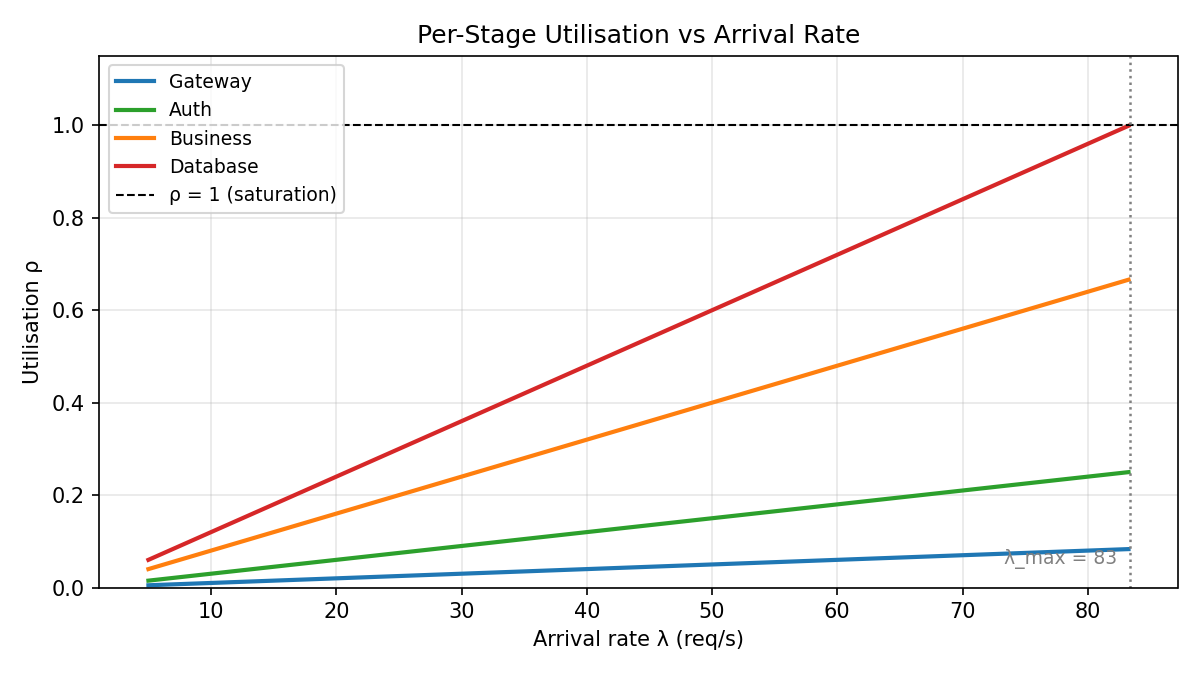
\includegraphics[width=0.82\textwidth]{../figures/fig1_utilisation.png}
  \caption{Per-stage utilisation $\rho_i = \lambda/\mu_i$ vs arrival rate.
           The Database line reaches $\rho = 1$ at $\lambda = \SI{83.3}{req/s}$,
           establishing it as the bottleneck. The target load of \SI{200}{req/s}
           lies far beyond all stable operating points shown.}
  \label{fig:util}
\end{figure}

The Database stage has the lowest service rate ($\mu_4 = \SI{83.3}{req/s}$) and reaches
saturation first. At the given $\lambda = \SI{200}{req/s}$:
\begin{align*}
  \rho_{\text{Gateway}}  &= 0.200, &
  \rho_{\text{Auth}}     &= 0.600, \\
  \rho_{\text{Business}} &= 1.600 > 1 \quad \text{(unstable)}, &
  \rho_{\text{Database}} &= 2.400 > 1 \quad \text{(unstable)}.
\end{align*}
Both Business and Database are overloaded. The primary bottleneck is the Database
because it saturates at the lowest load, but any capacity plan must fix both.

\subsection{Latency and P95 vs arrival rate}

Figure~\ref{fig:latency_vs_lam} shows how mean E2E latency and P95 grow with $\lambda$
in the stable regime.

\begin{figure}[H]
  \centering
  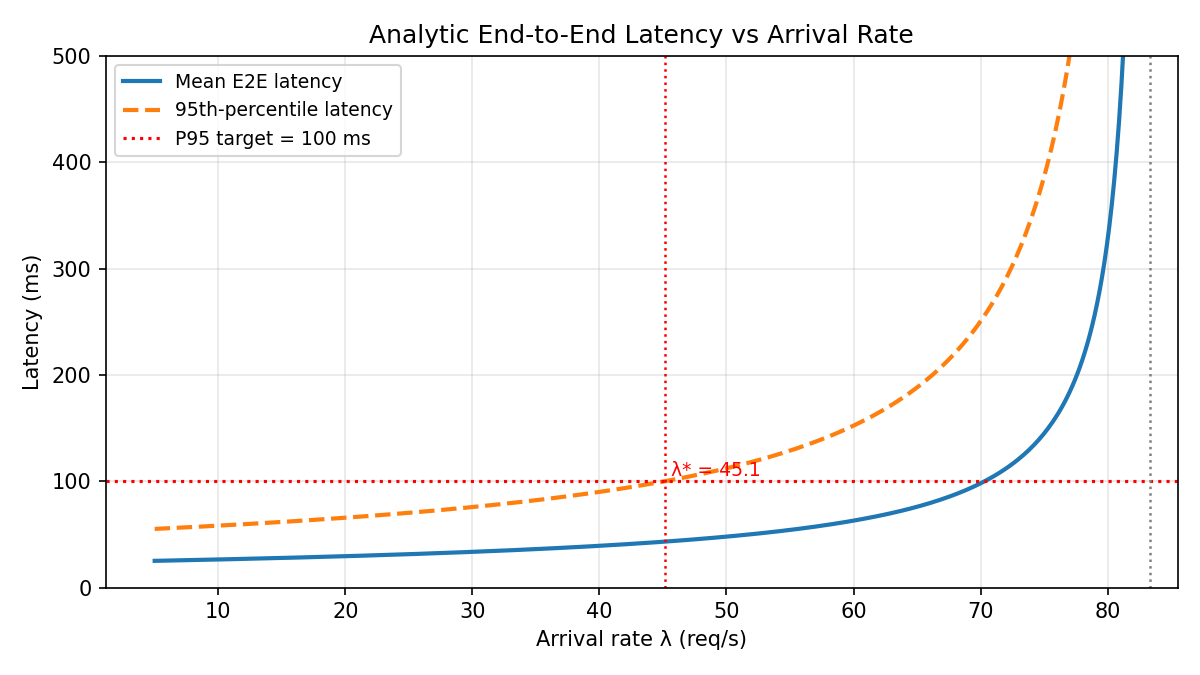
\includegraphics[width=0.82\textwidth]{../figures/fig2_latency_vs_lambda.png}
  \caption{Analytic mean and P95 end-to-end latency vs arrival rate under M/M/1
           assumptions. The 100\,ms P95 target (dashed red) is violated at
           $\lambda^* \approx \SI{45.1}{req/s}$, well below the stability limit of
           \SI{83.3}{req/s}.}
  \label{fig:latency_vs_lam}
\end{figure}

The P95 target of \SI{100}{ms} is violated at $\lambda^* = \SI{45.1}{req/s}$.
This means the current single-server architecture cannot serve even a quarter of the
target load within the latency SLA, let alone the full $\SI{200}{req/s}$.

At $\lambda = \SI{50}{req/s}$ (the reference stable point):
\[
  W = \SI{47.92}{ms}, \qquad t_{95} = \SI{112.18}{ms}.
\]
The breakdown of mean latency is: Gateway \SI{1.05}{ms} (2\%), Auth \SI{3.53}{ms} (7\%),
Business \SI{13.33}{ms} (28\%), Database \SI{30.00}{ms} (63\%). The Database stage
dominates even at moderate utilisation.

\subsection{P95 vs arrival rate: simulation across distributions}

Figure~\ref{fig:p95_vs_lam} compares the analytic P95 with simulated P95 for exponential
and lognormal service times across the stable $\lambda$ range.

\begin{figure}[H]
  \centering
  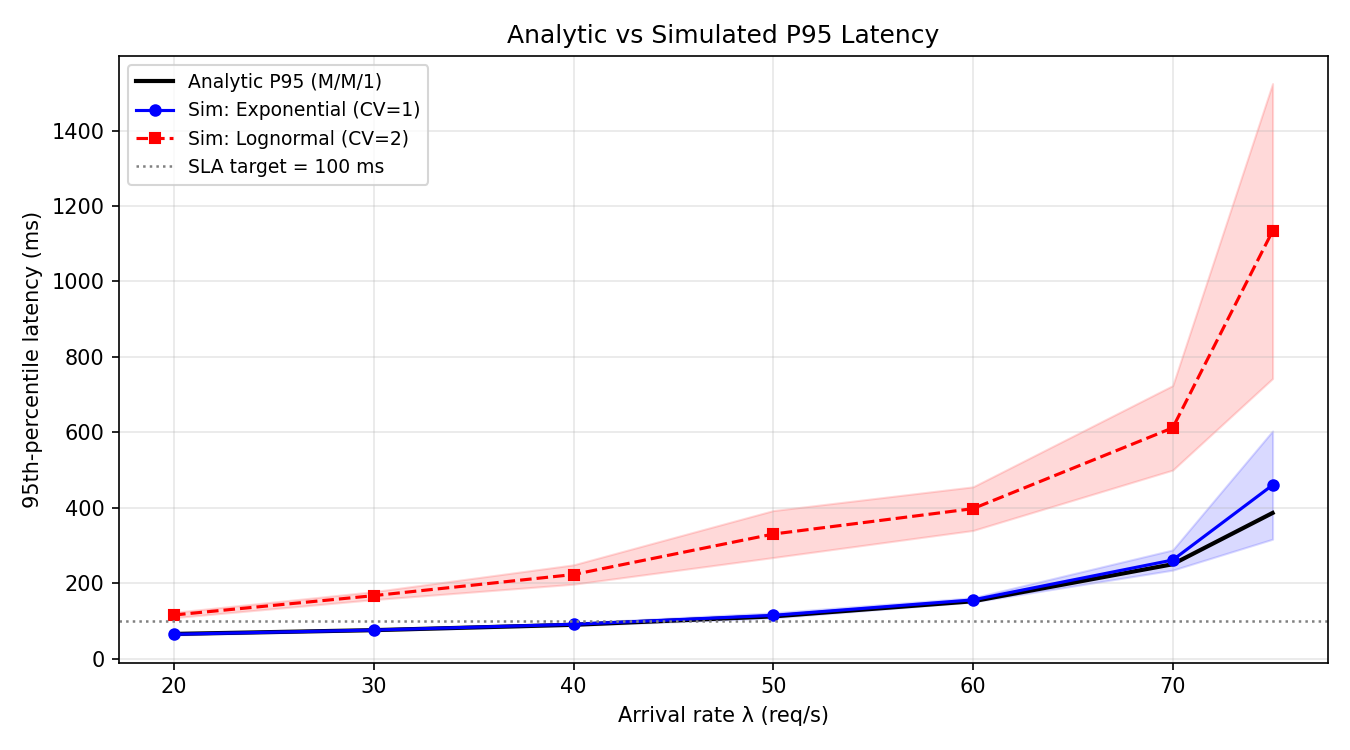
\includegraphics[width=0.88\textwidth]{../figures/fig5_p95_vs_lambda.png}
  \caption{Analytic P95 (black) and simulated P95 for exponential (blue, CI shown)
           and lognormal (red, CI shown) service times vs arrival rate.
           The SLA target of 100\,ms (grey dotted) is violated much earlier for
           lognormal service. Shaded bands are 95\% confidence intervals over 8 replications.}
  \label{fig:p95_vs_lam}
\end{figure}

The lognormal simulation diverges from the analytic curve at all loads, confirming that
the CV\,=\,1 assumption in the analytic model persistently underestimates tail latency.
For lognormal service (CV\,=\,2), the 100\,ms target is violated closer to $\lambda \approx \SI{30}{req/s}$.

\subsection{Part (e): Capacity strategy comparison}
\label{sec:capacity}

At $\lambda = \SI{200}{req/s}$, both Business and Database must be upgraded. The minimum
server counts for stability are:
\[
  N_{\text{Business}} \geq \left\lceil \frac{200}{125} \right\rceil + 1 = 3,
  \qquad
  N_{\text{Database}} \geq \left\lceil \frac{200}{83.3} \right\rceil + 1 = 4.
\]
Both strategies use the same total cost: $\Delta N = (3-1) + (4-1) = 5$ extra server units.

\paragraph{Strategy A: Replicate (M/M/N at overloaded stages).}
Business becomes M/M/3 ($\rho_{\text{per}} = 0.533$) and Database becomes M/M/4
($\rho_{\text{per}} = 0.600$). Using the Erlang-C formula~\eqref{eq:erlang_c}:
\[
  W_{\text{Business}}^{(A)} = \SI{9.56}{ms}, \quad
  W_{\text{Database}}^{(A)} = \SI{14.15}{ms}, \quad
  W^{(A)} = \SI{32.47}{ms}.
\]

\paragraph{Strategy B: Speed up (M/M/1 at higher rate).}
Business is upgraded by $3\times$ ($\mu_3' = \SI{375}{req/s}$, $s_3' = \SI{2.67}{ms}$,
$\rho = 0.533$) and Database by $4\times$ ($\mu_4' = \SI{333}{req/s}$, $s_4' = \SI{3}{ms}$,
$\rho = 0.600$). Using~\eqref{eq:mm1_W}:
\[
  W_{\text{Business}}^{(B)} = \SI{5.71}{ms}, \quad
  W_{\text{Database}}^{(B)} = \SI{7.50}{ms}, \quad
  W^{(B)} = \SI{21.96}{ms}.
\]

Figure~\ref{fig:capacity_bars} compares per-stage and total latency for both strategies.
Strategy B achieves a mean E2E latency \SI{10.5}{ms} (32\%) lower than Strategy A at
equal cost.

\begin{figure}[H]
  \centering
  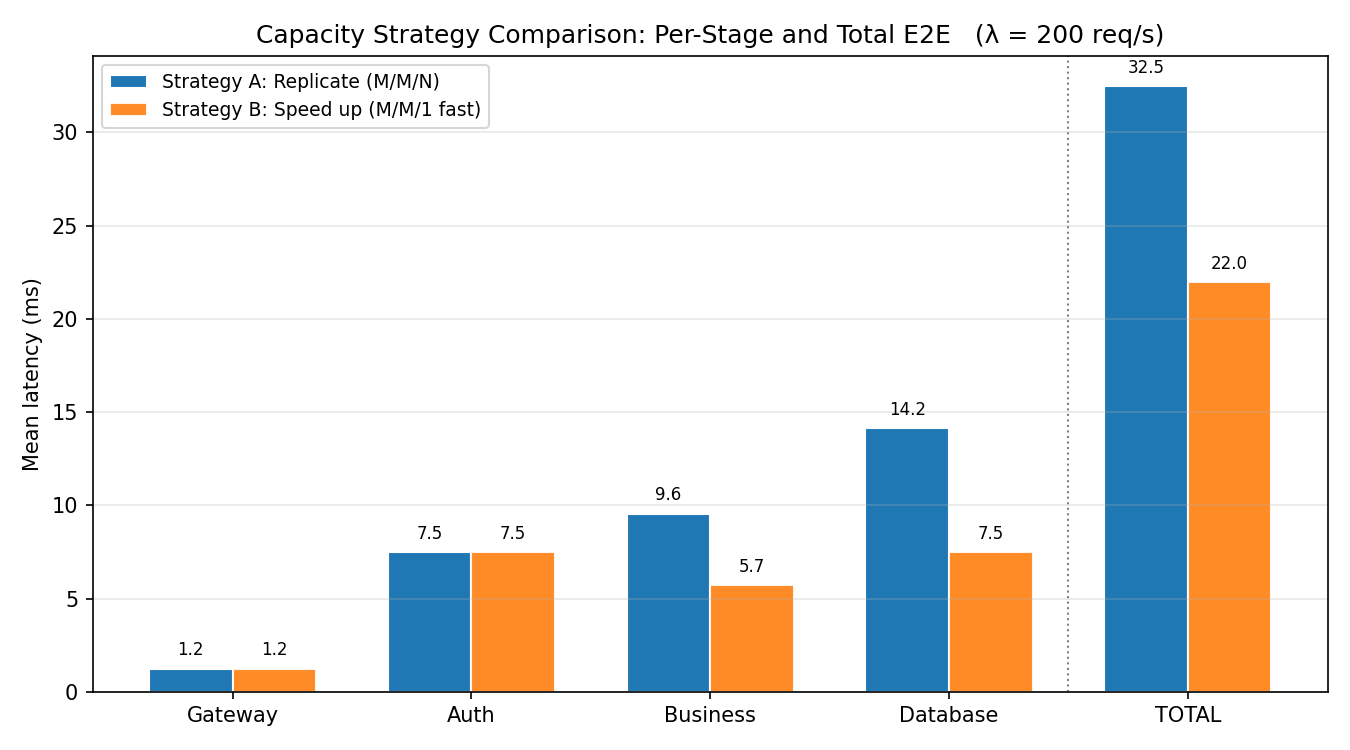
\includegraphics[width=0.88\textwidth]{../figures/fig7_capacity_strategies.png}
  \caption{Per-stage and total E2E mean latency for Strategy A (replicate, M/M/N)
           and Strategy B (speed up, M/M/1 faster). Equal cost of 5 extra server units.
           Strategy B dominates in every stage and in total.}
  \label{fig:capacity_bars}
\end{figure}

\paragraph{Why one fast server beats several slow ones.}
For a fixed offered load $a = \lambda/\mu$ and per-server utilisation $\rho = a/N$,
the M/M/1 model with rate $N\mu$ (one fast server) has mean sojourn:
\[
  W^{(B)} = \frac{1}{N\mu(1 - \rho)} = \frac{1}{N\mu - \lambda},
\]
while the M/M/N model with $N$ servers of rate $\mu$ has:
\[
  W^{(A)} = \frac{C(N, a)}{N\mu - \lambda} + \frac{1}{\mu}.
\]
Since $C(N,a) \geq 0$ and $1/\mu > 0$, we always have $W^{(A)} \geq W^{(B)}$.
The gap arises because $N$ slower servers create coordination overhead: a request may
arrive when all servers are busy even if their total capacity exceeds the load.
A single fast server has no such overhead and also eliminates the need for a load balancer.

Figure~\ref{fig:capacity_cdf} shows simulated empirical CDFs confirming the analytic result.

\begin{figure}[H]
  \centering
  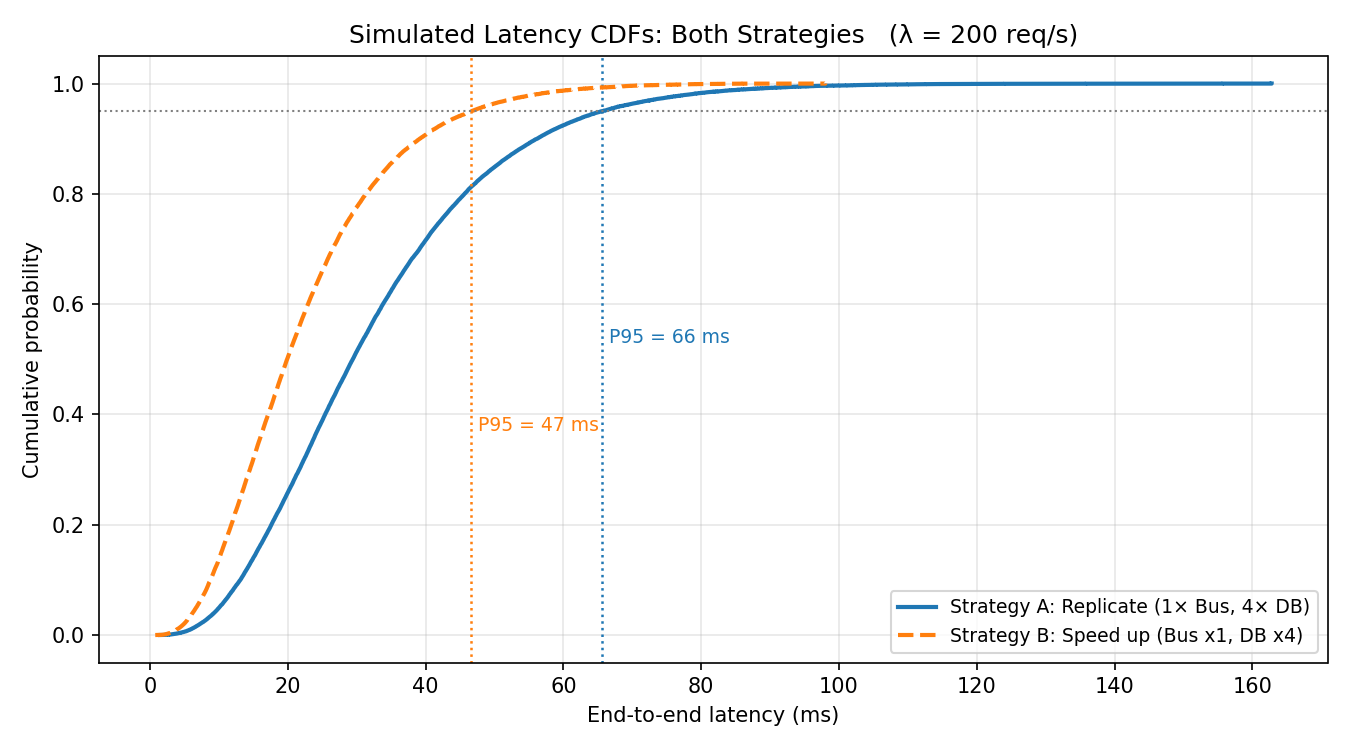
\includegraphics[width=0.88\textwidth]{../figures/fig8_capacity_sim.png}
  \caption{Empirical latency CDFs from simulation at $\lambda = \SI{200}{req/s}$
           for both strategies (exponential service times). Strategy B (orange dashed)
           achieves lower P95 and a lighter tail than Strategy A (blue solid).}
  \label{fig:capacity_cdf}
\end{figure}

\paragraph{Recommendation.}
Adopt \textbf{Strategy B} (service-time reduction). At equal cost it reduces mean E2E
latency by 32\% and reduces P95 latency (as confirmed by simulation). Strategy A
(replication) has the advantage of fault tolerance (a single server failure in
Strategy B takes the stage offline), but this is an operational concern outside the
scope of the latency model.

% ============================================================
\section{Critical Evaluation}
\label{sec:critical}

\subsection{Where the model succeeds}

The M/M/1 / Jackson model works well for:
\begin{itemize}
  \item Identifying the bottleneck stage analytically with zero computation (simply
        compare $\mu_i$).
  \item Providing a closed-form lower bound on mean and P95 latency.
  \item Sensitivity analysis: the formula $W_i = s_i/(1-\rho_i)$ makes it immediate that
        a 10\% reduction in $s_4$ at $\rho_4 = 0.8$ reduces $W_4$ by 33\%, not 10\%.
  \item Capacity planning ratios: the equal-cost comparison is tractable analytically.
\end{itemize}

\subsection{Principal limitations}

\paragraph{Exponential service-time assumption (A2).}
This is the dominant source of error. The lognormal simulation shows P95 is 178\% higher
than the analytic prediction at $\lambda = 50$ req/s. Database service times are bimodal in practice: cache hits settle around 1--2\,ms
while index misses stretch to 10--50\,ms, giving CV\,$\gg$\,1. The M/M/1 model
is therefore a best-case lower bound on P95.

\paragraph{Independence assumption (A3).}
Jackson's theorem requires that no resource is shared between stages. In a real
microservice deployment, all four services may run on the same Kubernetes node and share
CPU, memory bandwidth, and network card. Under such conditions, a spike in one service
can degrade all others simultaneously. The product-form model then over-predicts performance.

\paragraph{Open-loop model (A5).}
The model assumes requests arrive regardless of system state. Under overload, real clients
implement timeouts and retries. Retried requests increase the effective arrival rate,
which creates a positive feedback loop that can cause cascading failure. The model cannot
predict or represent this regime.

\paragraph{No spatial or temporal heterogeneity.}
The model uses a single mean service time per stage. Real systems have diurnal load
patterns, version-dependent service rates, and cache warming effects. A single operating
point is insufficient for capacity planning over a full day.

\subsection{Next steps}

\begin{enumerate}
  \item \textbf{Measure service-time CVs in production.} The most useful single measurement
    is the empirical CV of Database service times. Even a rough estimate ($\pm$20\%)
    would let the lognormal simulation be calibrated to real data rather than the assumed
    CV\,=\,2.
  \item \textbf{Extend to G/G/1 (Kingman's approximation).} For general arrival and service
    processes, Kingman's formula provides a closed-form approximation:
    \[
      W_q \approx \frac{\rho}{1-\rho}\cdot\frac{c_a^2 + c_s^2}{2} \cdot \frac{1}{\mu},
    \]
    where $c_a, c_s$ are the CVs of inter-arrival and service times. This would replace
    the exponential assumption with measured CVs.
  \item \textbf{Model shared-resource contention.} If stages co-locate on the same host,
    a coupled model (closed queueing network or simulation with shared CPU pool) is needed.
  \item \textbf{Add timeout and retry logic.} A non-linear ODE or Markov chain model
    capturing retry amplification would reveal the actual collapse point under overload.
\end{enumerate}

\subsection{What I would not trust this model for}

\begin{itemize}
  \item Predicting P99 or higher percentiles (the tail is exponential under M/M/1 but
    power-law in practice).
  \item Planning for flash-crowd or correlated arrival events.
  \item Making deployment decisions without validating service-time CVs against production
    traces.
\end{itemize}

% ============================================================
\section*{Use of AI Tools}

GitHub Copilot was used as a coding assistant to identify syntax errors during
implementation. All writing, modelling decisions, mathematical derivations,
analysis, and conclusions are the author's own.

% ============================================================
\section*{Reproducibility Statement}

All results are produced by running \texttt{python main.py} from the \texttt{Problem\,13/}
directory with \texttt{requirements.txt} satisfied. The analytic code is fully deterministic.
The simulation uses \texttt{numpy.random.default\_rng(seed)} with seeds 1000--1007;
the base seed is declared in \texttt{simulation.py} line 32.


% ============================================================
\begin{thebibliography}{9}

\bibitem{jackson1957}
J.~R. Jackson,
``Networks of Waiting Lines,''
\textit{Operations Research}, vol.~5, no.~4, pp.~518--521, 1957.

\bibitem{latouche1999}
G.~Latouche and V.~Ramaswami,
\textit{Introduction to Matrix Analytic Methods in Stochastic Modeling}.
SIAM, Philadelphia, 1999.

\bibitem{harchol2013}
M.~Harchol-Balter,
\textit{Performance Modeling and Design of Computer Systems}.
Cambridge University Press, 2013.

\bibitem{little1961}
J.~D.~C. Little,
``A Proof for the Queuing Formula: $L = \lambda W$,''
\textit{Operations Research}, vol.~9, no.~3, pp.~383--387, 1961.

\bibitem{dean2013}
J.~Dean and L.~A. Barroso,
``The Tail at Scale,''
\textit{Communications of the ACM}, vol.~56, no.~2, pp.~74--80, 2013.

\bibitem{kleinrock1975}
L.~Kleinrock,
\textit{Queueing Systems, Volume~1: Theory}.
Wiley-Interscience, New York, 1975.

\end{thebibliography}

\end{document}
